\documentclass{cornell}
\usepackage{lipsum}
\begin{document} 

\title{
    \vspace{-3em}
        \begin{tcolorbox}[colframe=white,opacityback=0]
            \begin{tcolorbox}
                \Huge\sffamily "The Evolution of Physics", EINSTEIN, Albert and INFELD, Leopold, 2008, Zahar
            \end{tcolorbox}
        \end{tcolorbox}
    \vspace{-3em}
}
\maketitle

\begin{tcolorbox}
\preread{I read the Portuguese(Brazilian) version of this book, in 2014. I can't remember if I had any goals when reading this book or if I just randomly select something to read at the bookshop.}{Sometimes I get tired about reading recreational mathematics, so i jump into physics books.}
\end{tcolorbox}


\noindent
It turns out this was one of the best physics books that I have ever had. And just after starting it, I noticed Einstein was one of the authors! This book has four parts, explaining part of the motivations for some of the ideas in physics. It also explains how some pieces were connected to reach the scenario we have nowadays. I got interesting insights after reading this book.

%\begin{tcolorbox}[colback=white,opacityframe=0]
\topic{Part I - the Rise of the mechanical view}%
{Mystery and clues. "The scientist that read the book of Nature [...] must find his own solution". One of the early mysteries was related to motion. Our intuition would tell us that the speed is related to the action. Inertia and the uniform movement (that's a simple way to start). Galileo notices that some sort of force can change the speed of an object (acceleration). There's a connection between a force and the change of the speed (and Newton comes up with a formula). Force: an action over a body. Putting aside the movement over a straight line, let's take a look at curves, which are slightly more complicated. Example of a sphere - we give it an initial impulse and it moves. Its direction can also change. A force can change the sphere's speed as well as its direction, and that's one of the reasons vectors are important. We can now represent a force and a change on the speed. "A force and the change of the speed are vectors with the same direction". We can take qualitative conclusions about physics [observing patterns] and quantitative ones (we need some help from mathematics). Newton's law of gravitation is about a force, gravity. That's an interesting force, especially because we can see the moon and the stars. }%
{We have the ability to imagine new scenarios, and this skill may be useful for physics. A new clue: the mass. The speed is related to the mass of the body. Inertial mass and gravitational mass. There were other clues to follow - the heat. Is it a substance? There's a difference between temperature and heat. The heat is like the mass, but they are not the same kind of thing. So how do explain the heat? Proposal: create a 'theory of substances' to try to explain such concept. It worked for a while, until Rumford show a counterexample - the heat flows. Next, let's take a look at transformation. We can transform kinetic energy into potential energy. There's a transformation rate, that we can measure and determine the conservation of the energy in a closed system. Philosophy also influenced physics (ex: Democritus). Can we describe the entire Universe only with the Motion laws and the heat? No. There are different kinds of forces: attraction and repulsion. There were much more to come, such as the kinetic theory of the matter. How does it work on fluids? (on a gas, for example). We must take a look at small portions of the matter, the molecules. We can't see such structure, but we created accurate representations of it. }%
%\end{tcolorbox}
{Further reference: Helmholtz}%

\begin{tcolorbox}
\insight{Vectors can carry more information than a scalar. We built a structure with a powerful communication channel. }
\end{tcolorbox}


%\begin{tcolorbox}[colback=white,opacityframe=0]
\topic{Part II - The Decline of the Mechanical View}%
{Two electric fluids and the idea of positive and negative. Conductors and insulators. A  new mystery - the electrostatic. The first attempts try to use ideas from mechanics, but they do not seem to fit well for this new scenario. Coulomb shows there's a force, but different from gravity (which is always present), the electric force only exist when the bodies have some sort of charge. The electric forces can be of attraction (such as gravity),  or repulsive. Do these structure have some sort of mass? It looks like they don't. An analogy - electric potential and temperature; electric charge - heat. I'll include an extra table, in Portuguese, with more analogies ( \ref{teof01}). This comparison is not very strict - if a hot body has contact with a cold body, the heat flows from the hotter to the colder. Opposite charges of equal magnitude cancel themselves. How does it happen? There must be a flow. We shall investigate the possibilities. We can take a guess - it flows from the higher electric potential to the lower electric potential. It's time to take a look at magnets.}%
%\end{tcolorbox}
{It looks like they have another distinct behaviour. They have poles (and they are magnetic dipoles). They seem to have a replication property - break a magnet in the middle and you obtain two magnets. And we see again the idea of attraction and repulsion, all based on the distance of the elements. Volta and his battery. The difference of potential creates a flow of 'something' from the higher potential to the lower potential. We observe heat on the wire. Different types of energy turning into some other type. Oersted. The unexpected relation between electricity and magnetism. There's another element not previously discussed: the light. What's the speed of the light? Galileo could not measure it. Fizeau took the measurements many years later. Is the light a type of substance? It travels following a straight line in the vacuum; if it goes through another body, we observe the refraction. It looks like there are small bodies of light that follow a straight path and change their direction if they collide against a body. This explanation was good enough for some scenarios. But what about the colours? Newton determined the visible spectrum of the light. Would the previous theory of small bodies of the light explain the colours? Maybe another component was necessary - the idea of waves. The obvious way to describe a wave is to look at the water and its behaviour, or thing about music. We can find the concept of wave length. There's more than one type of wave - longitudinal and transverse. Soon, Huygens described the light under the ideas of the behaviour of waves, spreading the wave theory of the light. \ref{teof02} shows a good comparison (in Portuguese) of the two attempts to describe the behaviour of the light. If the light a longitudinal of transverse wave? A new theory comes in - there must be a 'jelly' around the planets, which was called Ether. That would be the responsible transport element for the light. But describing the ether in terms of mechanics was painful. Something was not right. }%
{Further reference: Galileo "Two new Sciences"}%


\topic{Part III - Field, Relativity}%
{New ideas based on the results of Faraday, Maxwell and Hertz. Representing the fields as vectors, or lines of force. A field allow us to determine the forces acting in a magnetic dipole in other parts of the space. The current is always associated to a magnetic field. A force acts over a magnetic field when we put it next to a wire with a current. We must create a representation of the shape of this field. There will be closed lines (see solenoid). For the positive electric charge, the arrows of the field point out; for the negative, they point in. The electrostatic, magnetic and gravitation field are different. If we change the electric by moving a particle, we obtain a magnetic field (see \ref{teof03}). Varying a magnetic field makes an electric field appear; the opposite is also true. The number of lines of force represents the how intense is the field. Maxwell come sup with a set of equations that represent the structure of these two fields (the electromagnetic field). Even though they may follow some similar principles, we can't really compare Maxwell's equations with the laws of Mechanics and motion. The electromagnetic fields depends on the neighbourhood and recent facts; the gravitational field is not like that. }%
{The field brings up the concept of electromagnetic wave. They carry information about the variation of the electromagnetic field they are into. It moves in the vacuum. We can follow these waves, not matter how their history is. These waves travel with the speed of light. Is the light an electromagnetic wave? There was a challenge to make the physicists accept the concept of field. The Earth is our system of coordinates. We should study the relationships between two coordinate systems - and the mechanical laws cannot be valid in two systems at the same time. That would imply in contradictions. We shall adopt one system to be valid and we call it intertial system. How can we determine which one is going to be the inertial system? The time should be the same for all the coordinate systems, but the speed and the positions are not, changing the transformation laws. Newton motion laws do not change, which means we are talking about a classical transformation. }%
{"One way to not listen to what someone says is running faster than the speed of the sound". Would it be valid for the light? What should we do with the theories about the ether? The speed of the light does not change among the coordinate systems. The theory of the ether stopped making sense. The scientists could not fit it. The speed of light wouldn't change in the vacuum. In two coordinate systems moving with the same speed towards each other, the mechanical laws are the same and it's impossible to distinguish the uniform movement if you are inside these systems. So that means we shall reject the idea of the classical transformation. There should be something else. The ideas of relativity come up, and these time the experiments would use different clocks to measure time. A new idea of representing space and time using four dimensions - they all vary. There is a funny dialogue in the book exploring answers with self-reference.  }%
{Further reference: Oersted, Rowland}%


\topic{Part IV - Quanta}%
{Interesting consideration about continuum pieces of matter that should be considered as quanta. A cent is an elementary quanta for money; we have something similar for particles. We can use the same idea for the light; see \ref{teof04}. There are phenomena that can be explained by the wave of light, but not by the quantum theory and vice versa. Every time we consider elements that are not continuum, we should talk about probabilities. }%


\begin{figure}[!t]
\centering
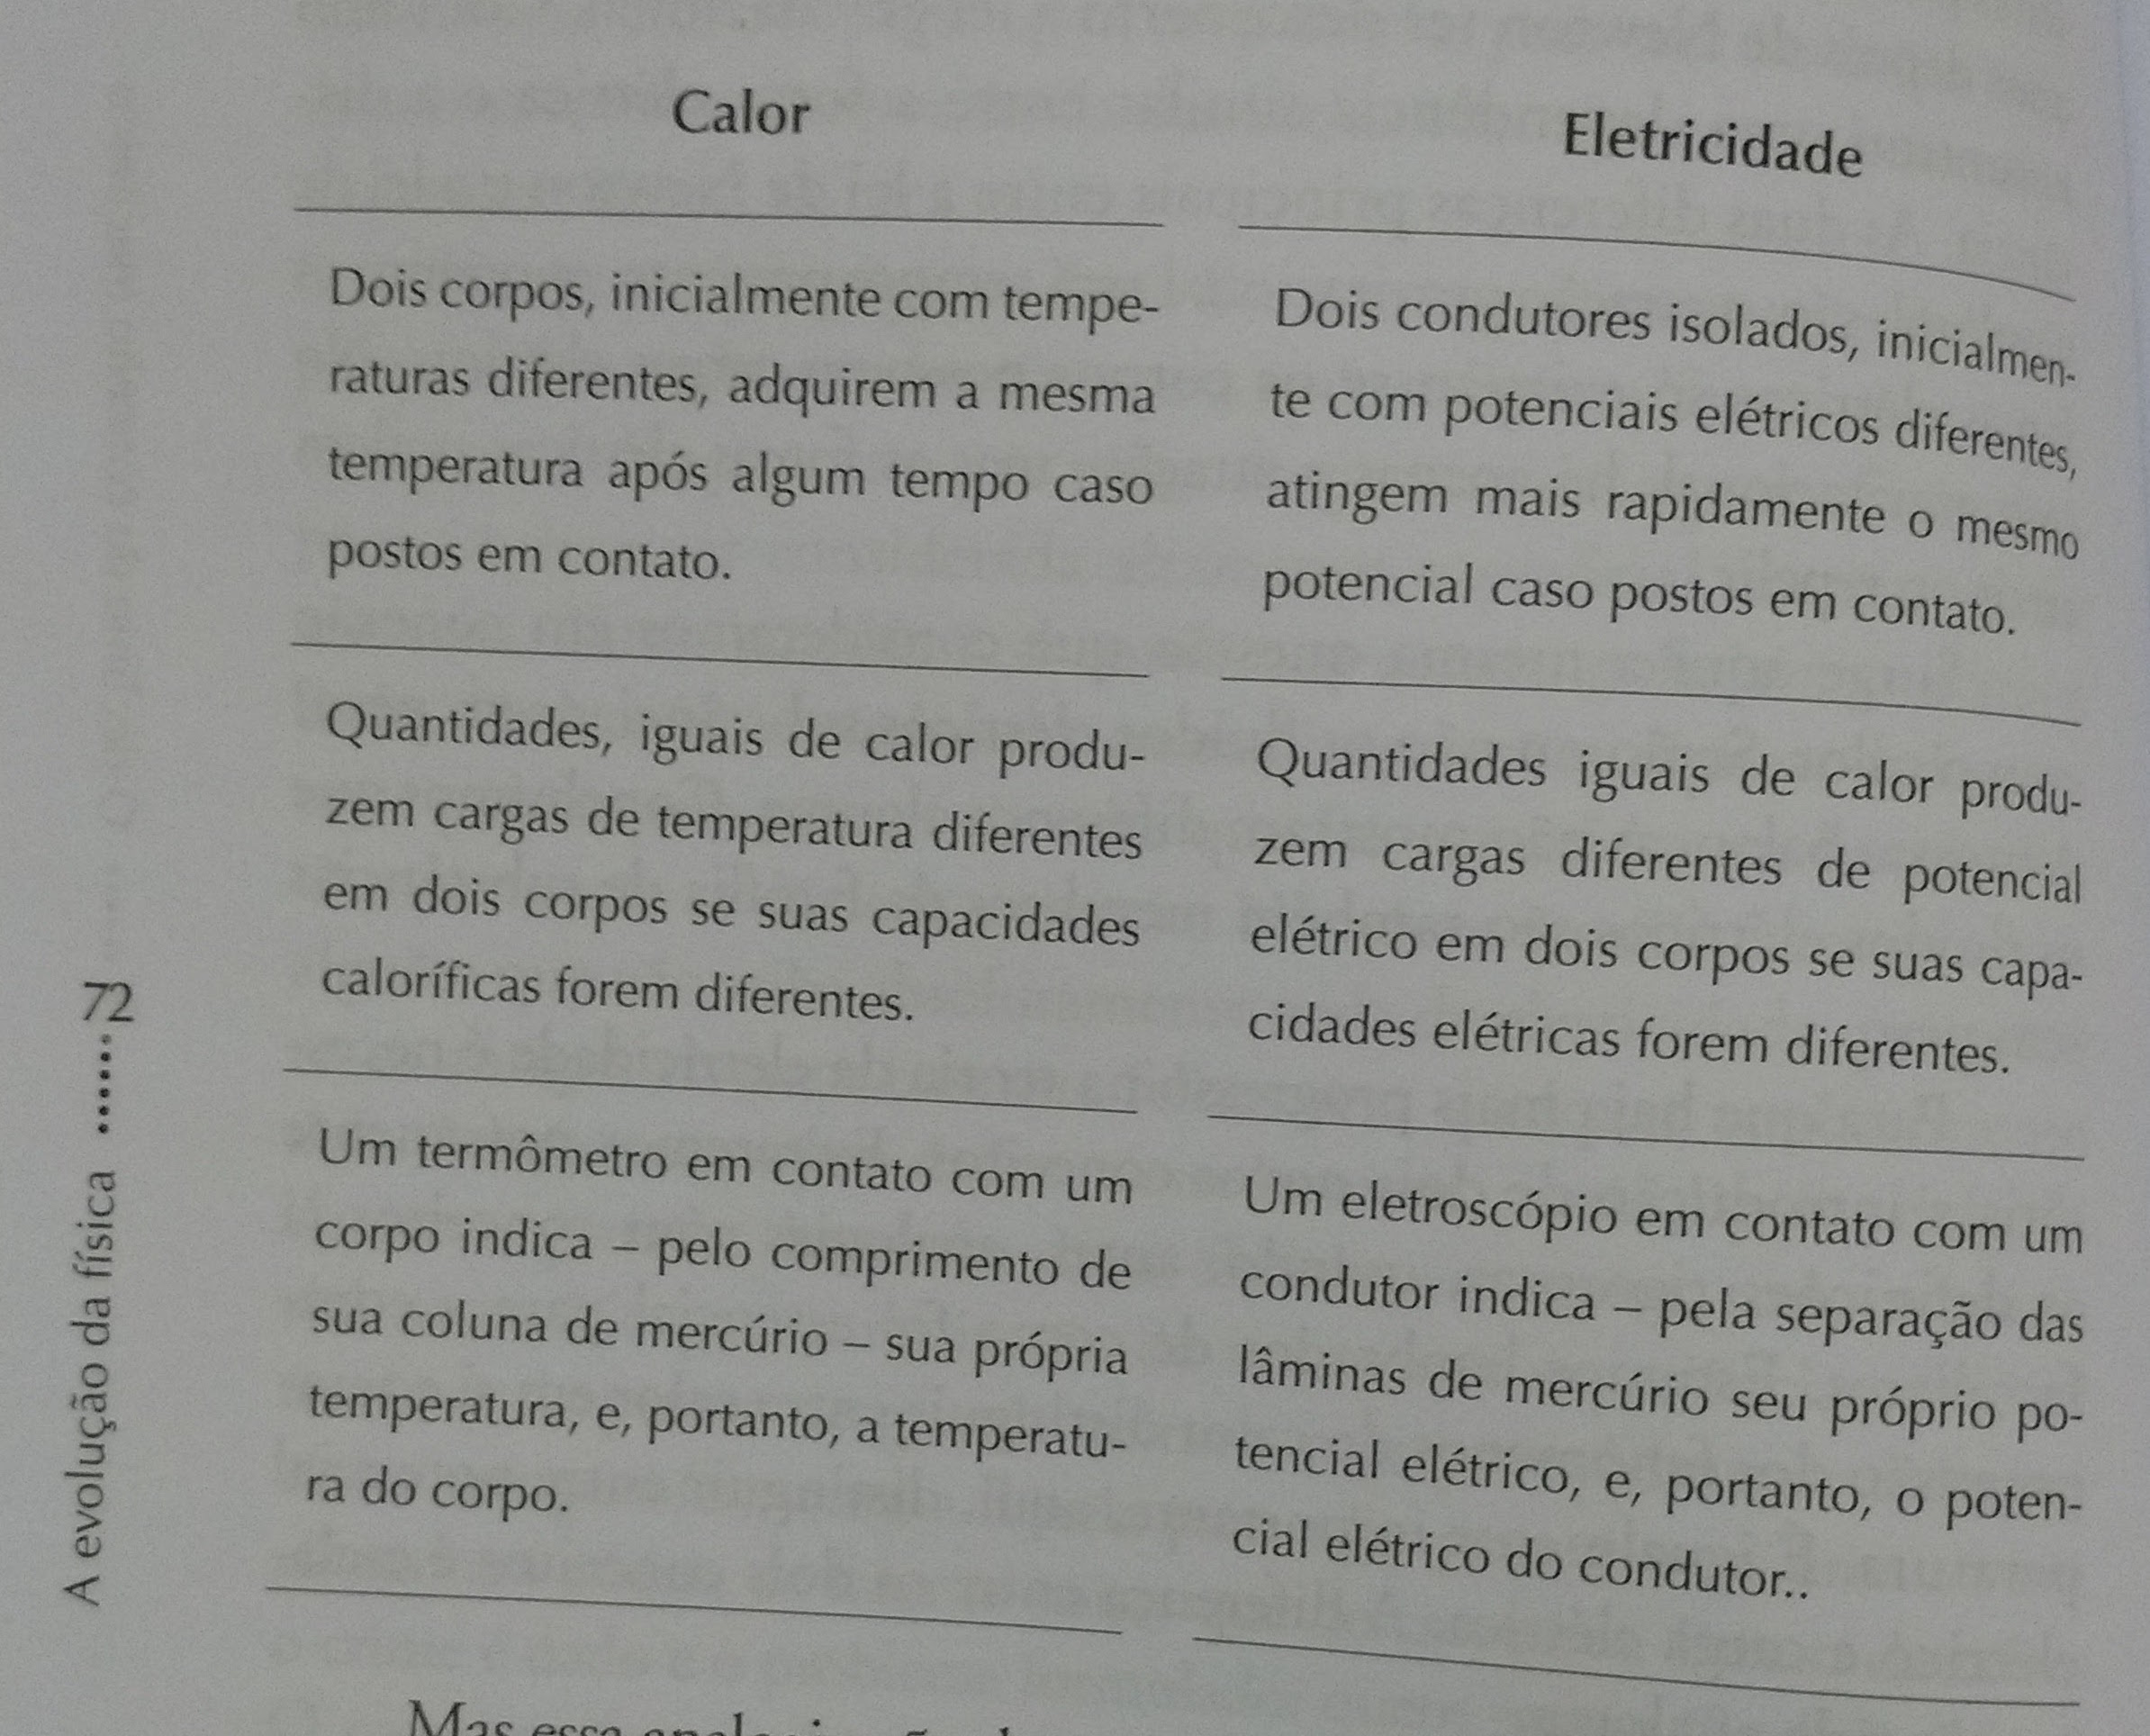
\includegraphics[width=1.0\linewidth]{images/teof01.jpg}
% where an .eps filename suffix will be assumed under latex, 
% and a .pdf suffix will be assumed for pdflatex; or what has been declared
% via \DeclareGraphicsExtensions.
\caption{Electricity and temperature }
\label{teof01}
\end{figure}


\begin{figure}[!t]
\centering
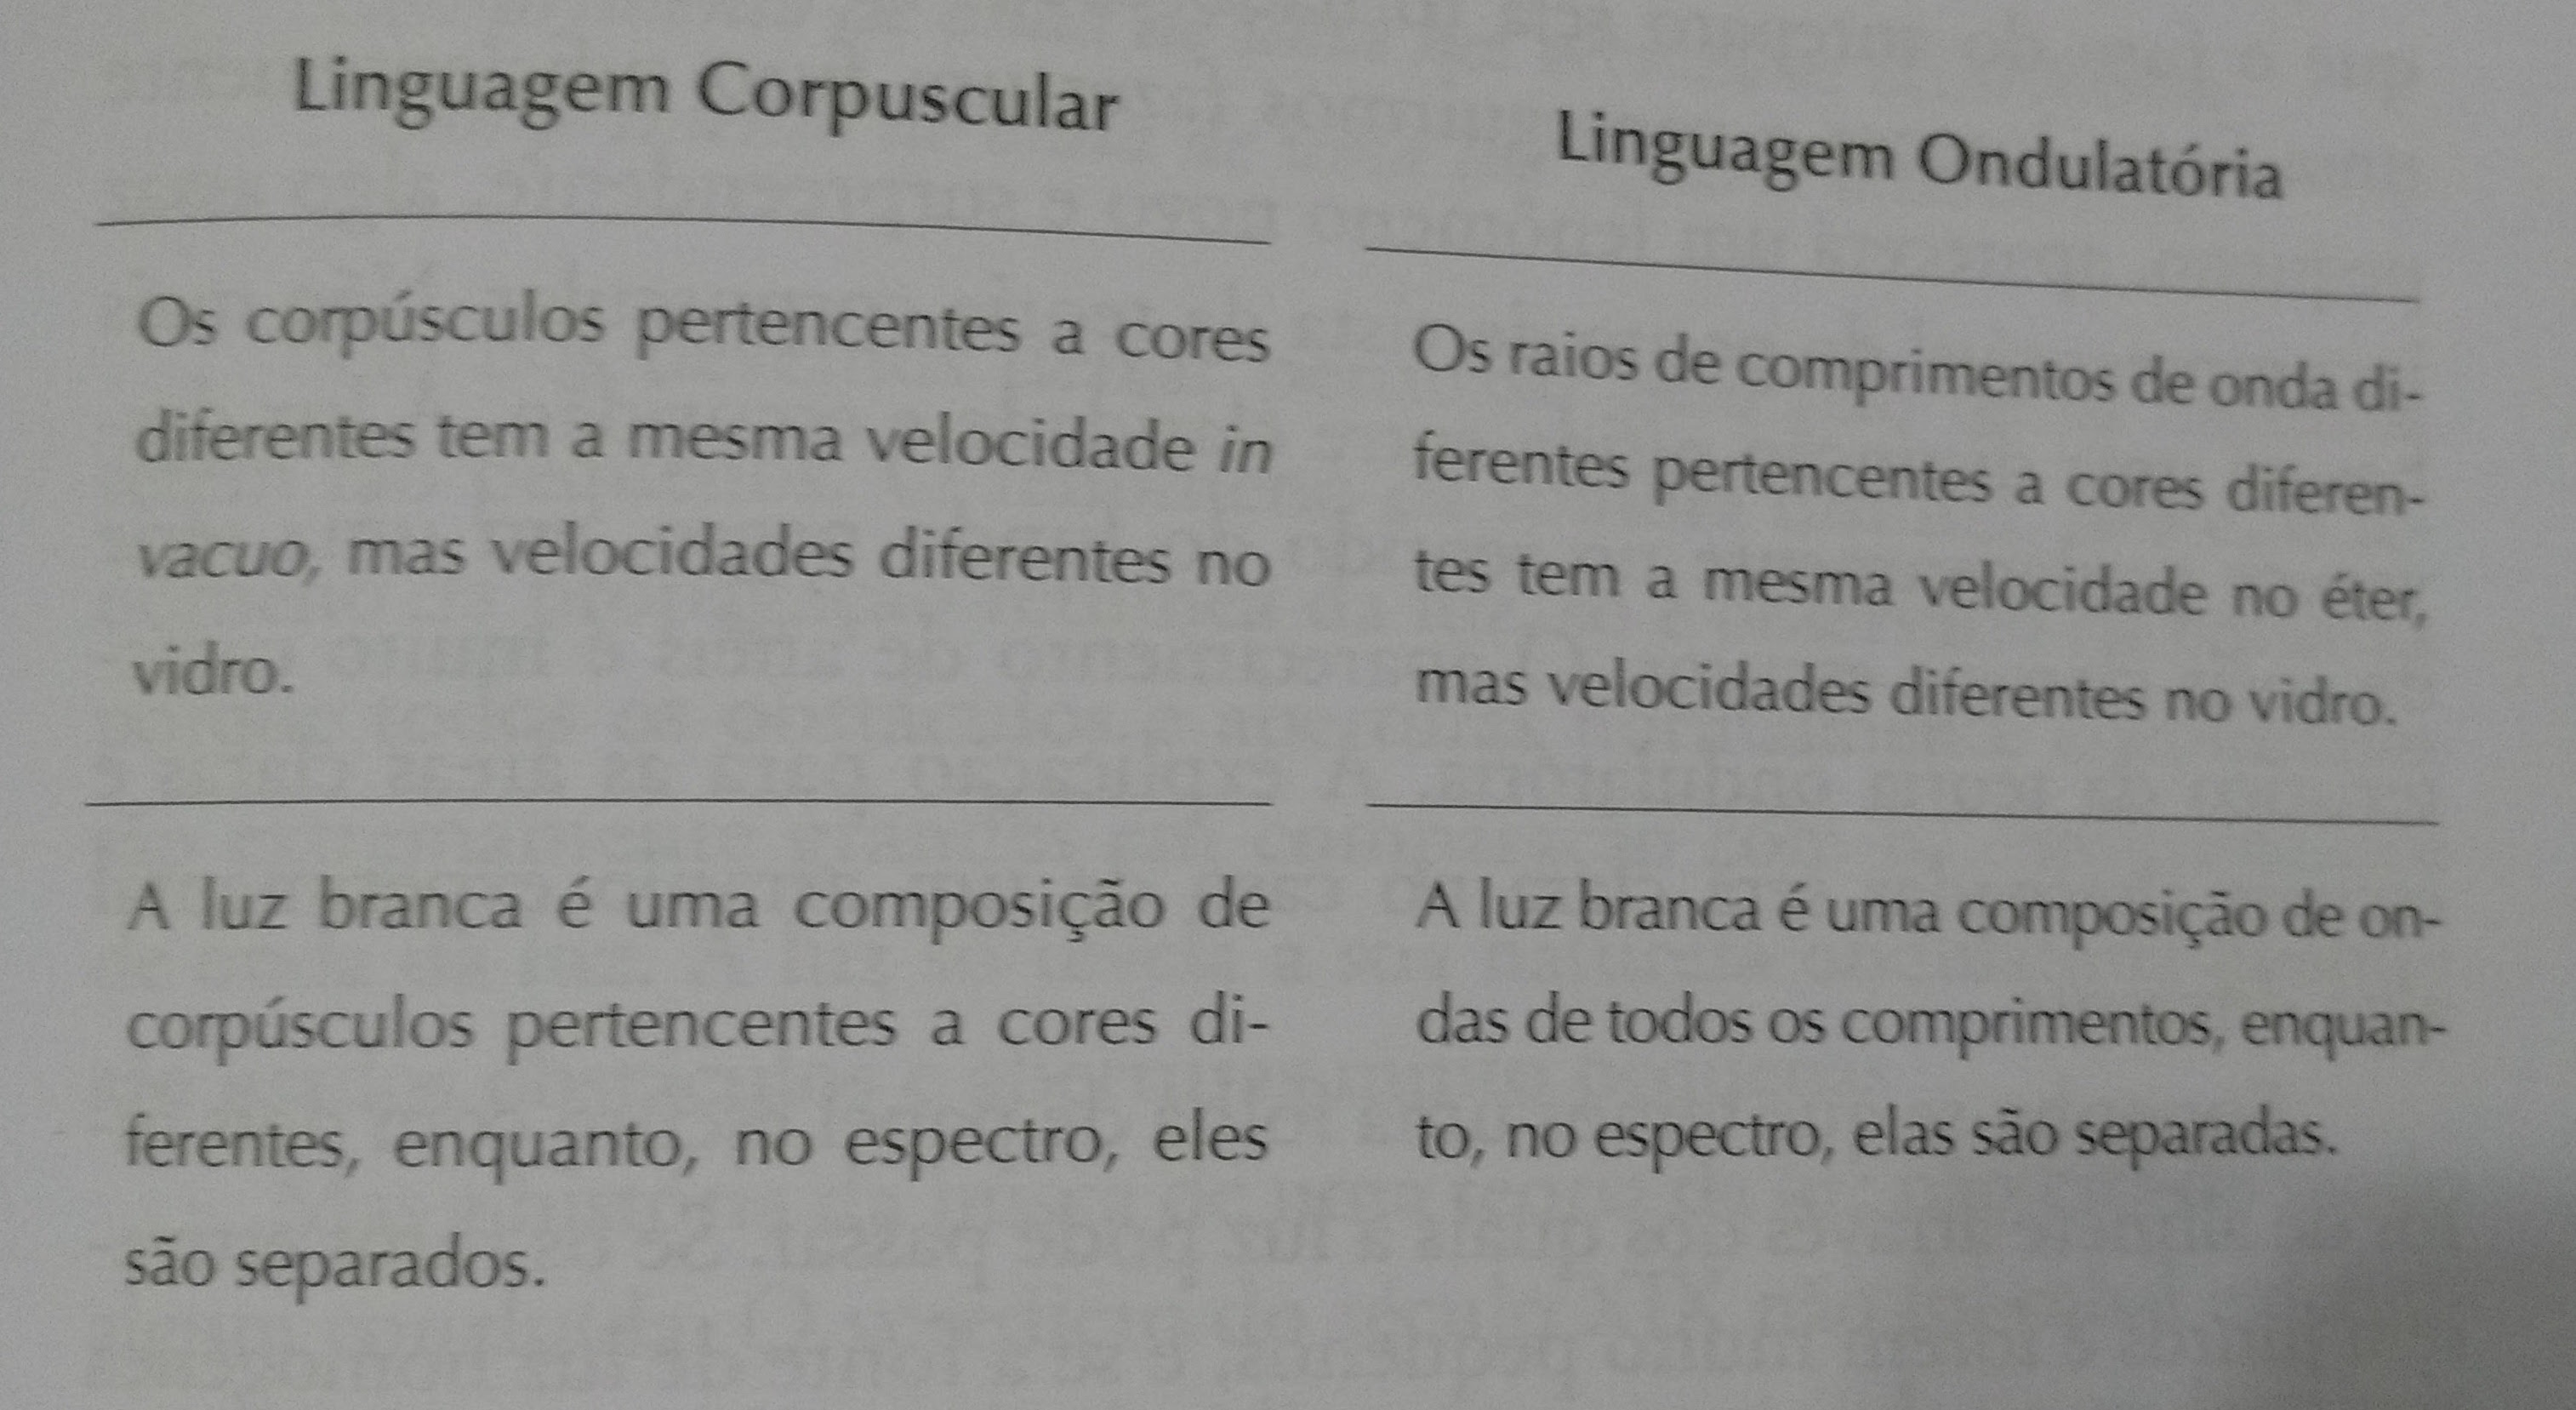
\includegraphics[width=1.0\linewidth]{images/teof02.jpg}
% where an .eps filename suffix will be assumed under latex, 
% and a .pdf suffix will be assumed for pdflatex; or what has been declared
% via \DeclareGraphicsExtensions.
\caption{Two behaviours of light }
\label{teof02}
\end{figure}


\begin{figure}[!t]
\centering
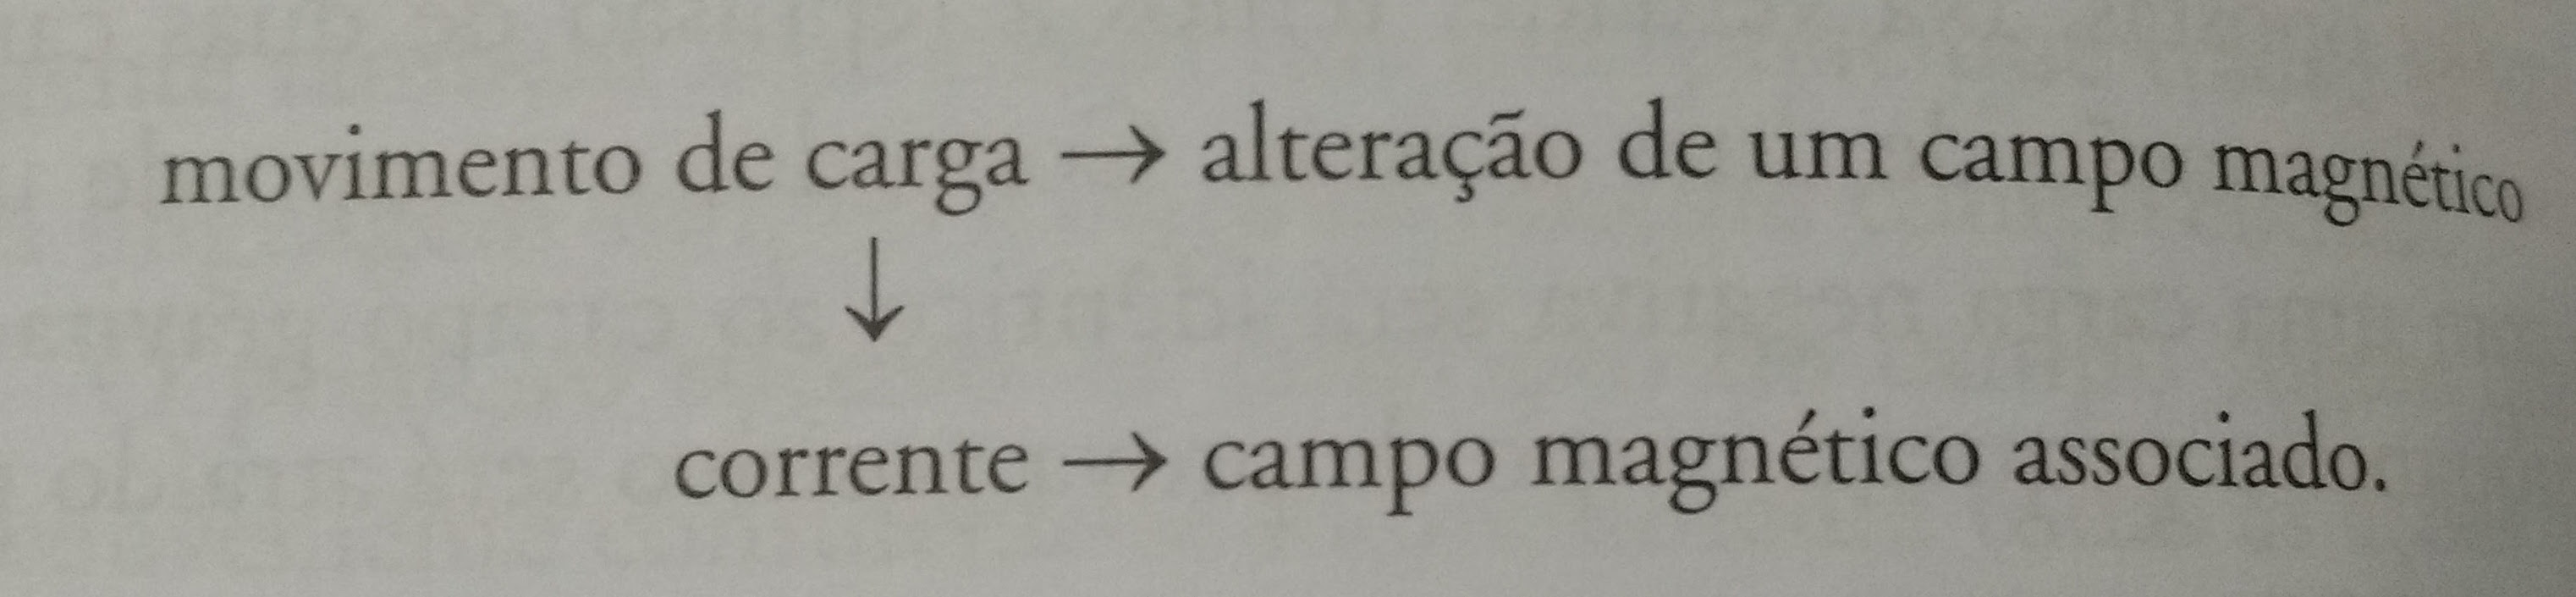
\includegraphics[width=1.0\linewidth]{images/teof03.jpg}
% where an .eps filename suffix will be assumed under latex, 
% and a .pdf suffix will be assumed for pdflatex; or what has been declared
% via \DeclareGraphicsExtensions.
\caption{Magnetic fields }
\label{teof03}
\end{figure}

\begin{figure}[!t]
\centering
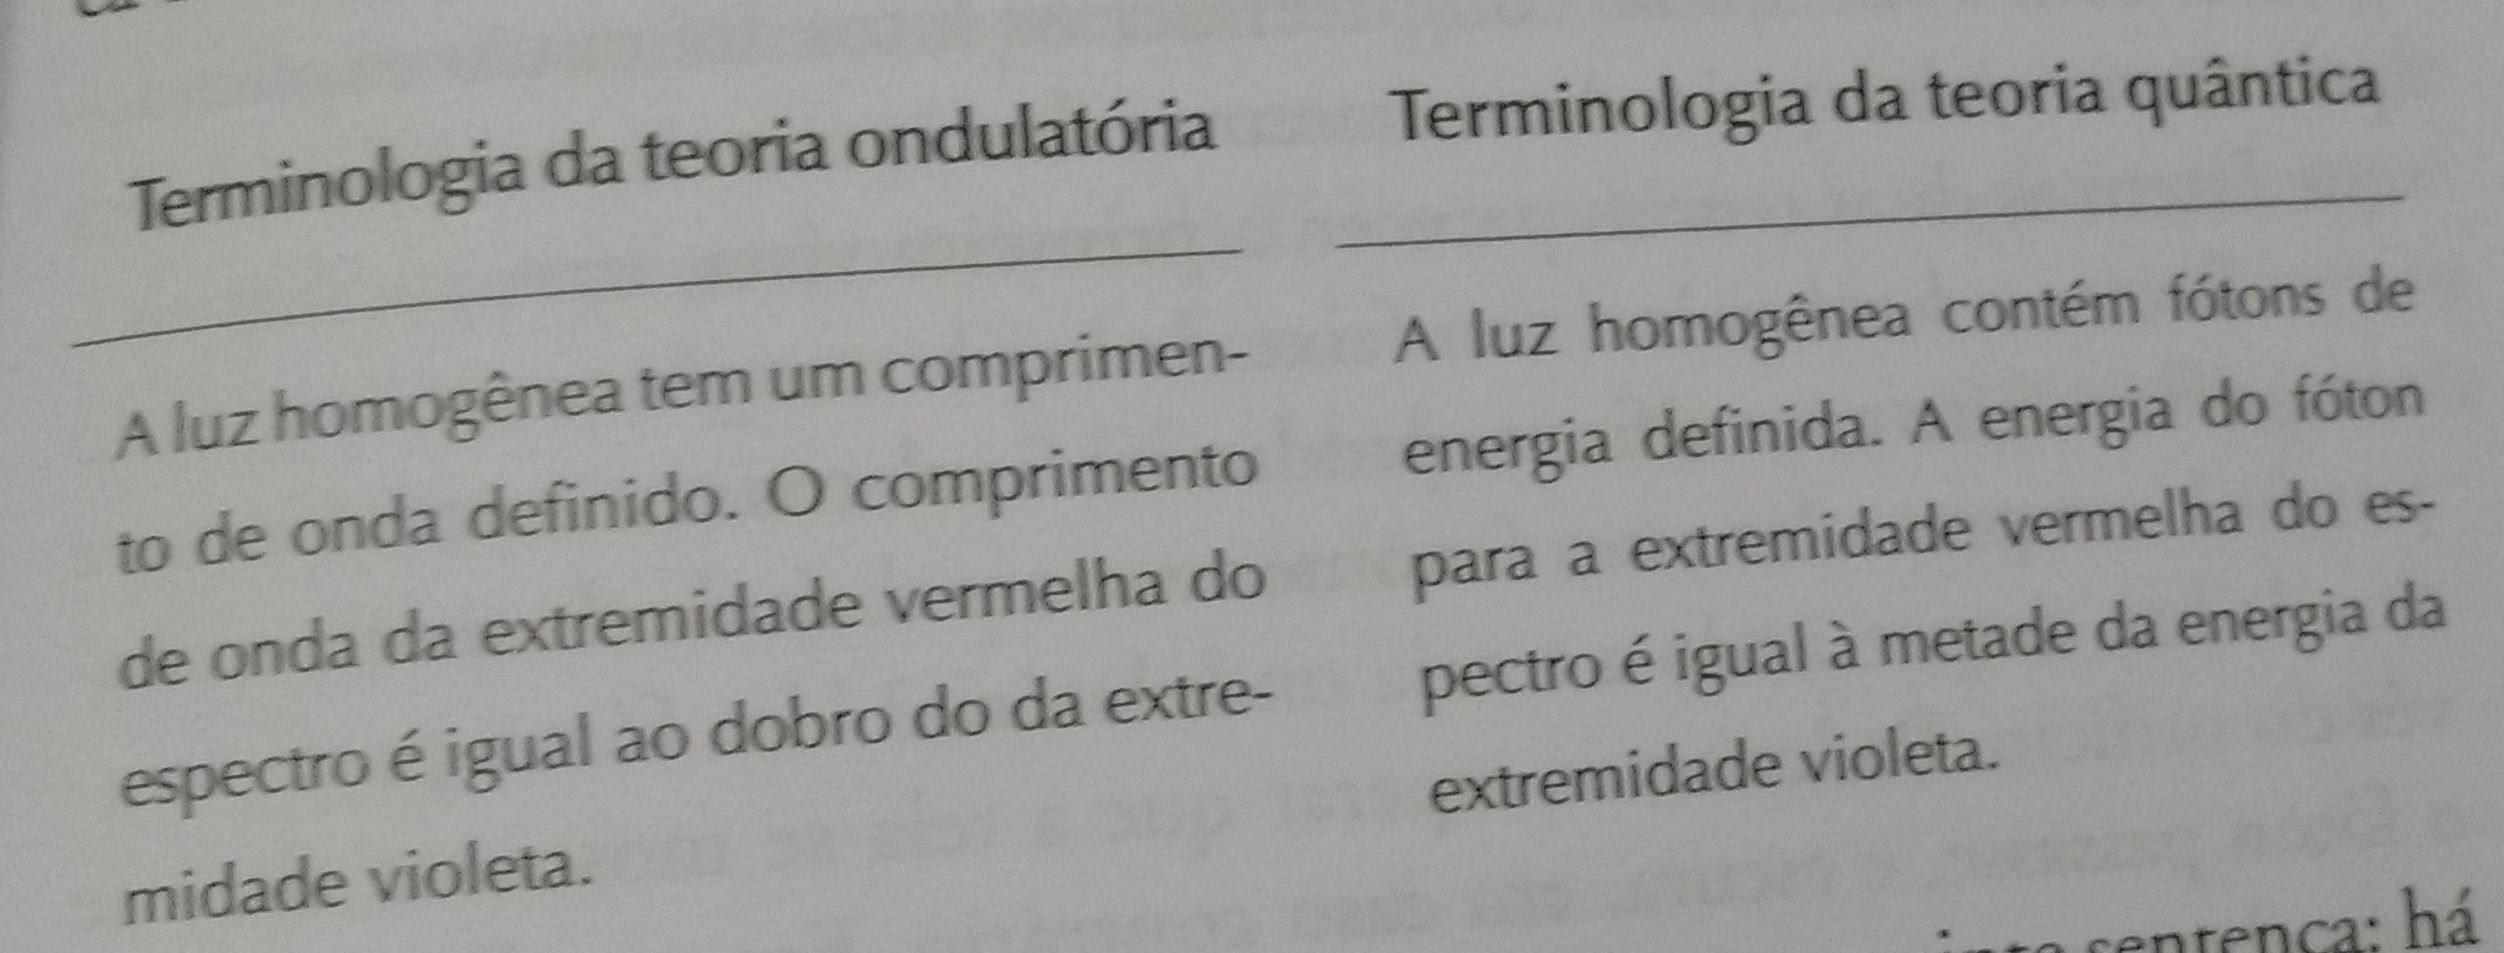
\includegraphics[width=1.0\linewidth]{images/teof04.jpg}
% where an .eps filename suffix will be assumed under latex, 
% and a .pdf suffix will be assumed for pdflatex; or what has been declared
% via \DeclareGraphicsExtensions.
\caption{Quantum vs. Wave }
\label{teof04}
\end{figure}

\summary{Brilliant examples. This book shows some of the paths the physicists took in order to build laws and theories for Physics. }



\end{document}